% Created 2026-05-20 Wed 14:21
% Intended LaTeX compiler: pdflatex
\documentclass[11pt, letterpaper]{article}

\usepackage[utf8]{inputenc}
\usepackage[T1]{fontenc}
\usepackage{graphicx}
\usepackage{longtable}
\usepackage{wrapfig}
\usepackage{rotating}
\usepackage[normalem]{ulem}
\usepackage{amsmath}
\usepackage{amssymb}
\usepackage{capt-of}
\usepackage{hyperref}
\usepackage[margin=2.5cm]{geometry}      % Márgenes decentes
\usepackage[utf8]{inputenc}
\usepackage{palatino}                   % Tipografía elegante
\usepackage{xcolor}                     % Colores personalizados
\author{Equipo Alpine White}
\date{\textit{{[}2026-04-20 Mon]}}
\title{Preparación para la Instalación Nativa de las distribuciones dadas.}
\hypersetup{
 pdfauthor={Equipo Alpine White},
 pdftitle={Preparación para la Instalación Nativa de las distribuciones dadas.},
 pdfkeywords={},
 pdfsubject={},
 pdfcreator={},
 pdflang={English}}
\begin{document}

\maketitle
\setcounter{tocdepth}{2}
\tableofcontents

\section{Información General}
\label{sec:org1bd62b8}
\begin{itemize}
\item \textbf{Equipo:}
\begin{itemize}
\item Arreguín Salgado Gael Emiliano
\item López Pérez Mariana
\item Nieto Gallegos Isaac Julián
\end{itemize}

\item \textbf{Distribución elegida:} Alpine Linux
\end{itemize}
\section{Alpine Linux}
\label{sec:orge4ef952}

\subsection{Despejar espacio para la instalación}
\label{sec:org57ecae9}

La instalación en bare metal de la distribución elegida se realizará sobre un equipo de cómputo del Laboratorio De Sistemas Operativos de la facultad.

Estos equipos tienen los siguientes medios de almacenamiento:

\begin{itemize}
\item Un disco NVME. Marcado como /dev/nvme0n1
\item Un disco de estado sólido. Marcado como /dev/sda
\end{itemize}

Al disco NVME no hay que tocar nada. Debemos reducir alguna de las particiones ya existentes en el disco de estado sólido para realizar nuestra instalación.

En mi caso concreto, reduje /dev/sda8 para obtener 160GB de espacio disponibles.

\begin{center}
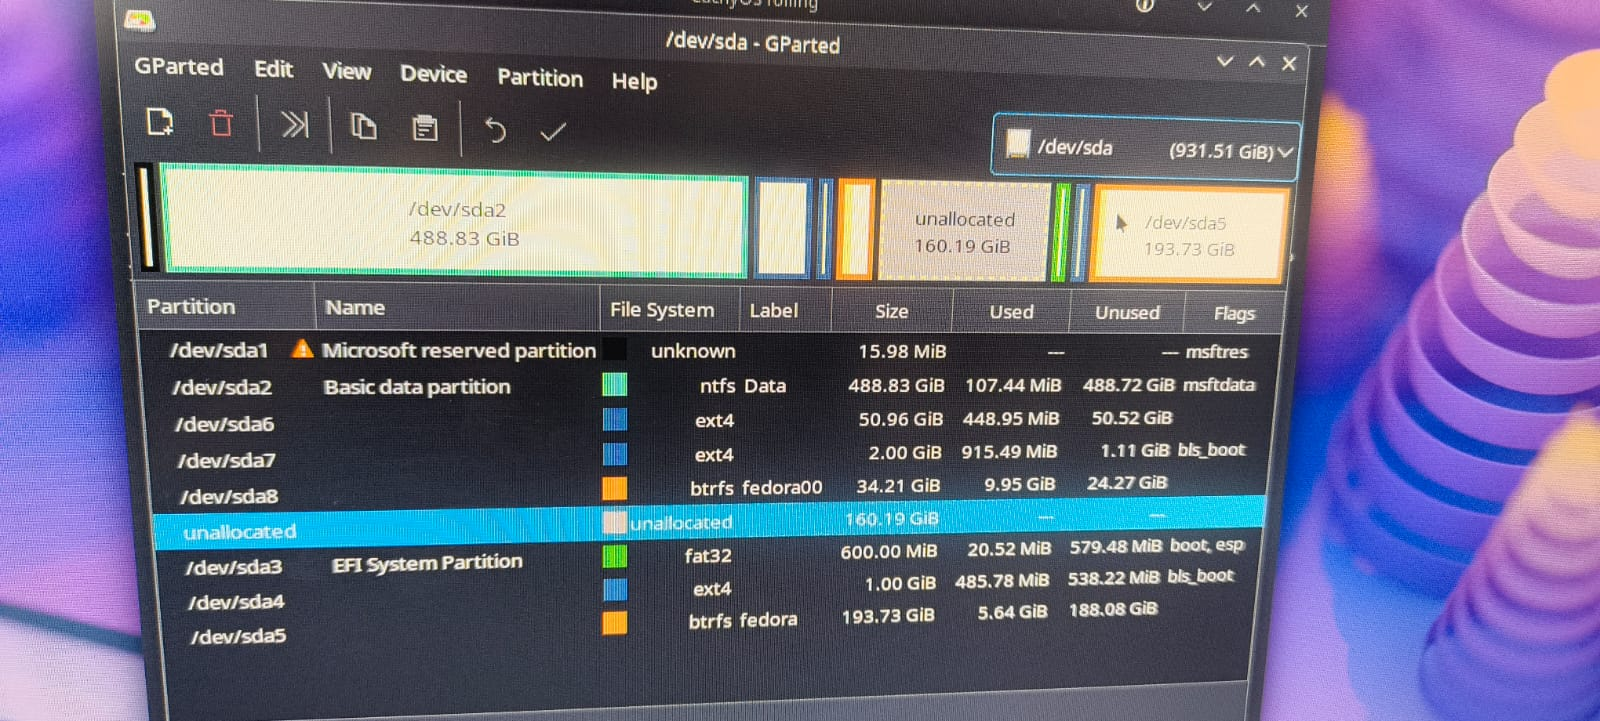
\includegraphics[width=.9\linewidth]{./1.jpg}
\end{center}
\subsection{Conexión a internet}
\label{sec:org58940df}

Alpine Linux viene con una instalación muy mínima por default. Por esto, vamos a necesitar descargar más herramientas de Internet. Evidentemente para esto, necesitamos conectarnos a internet.

Para esto, ejecutaremos un script integrado en Alpine llamado \textbf{setup-interfaces}. Ya que necesitamos conectarnos por Ethernet, las opciones por default nos resultan suficientes para esto.

\begin{center}
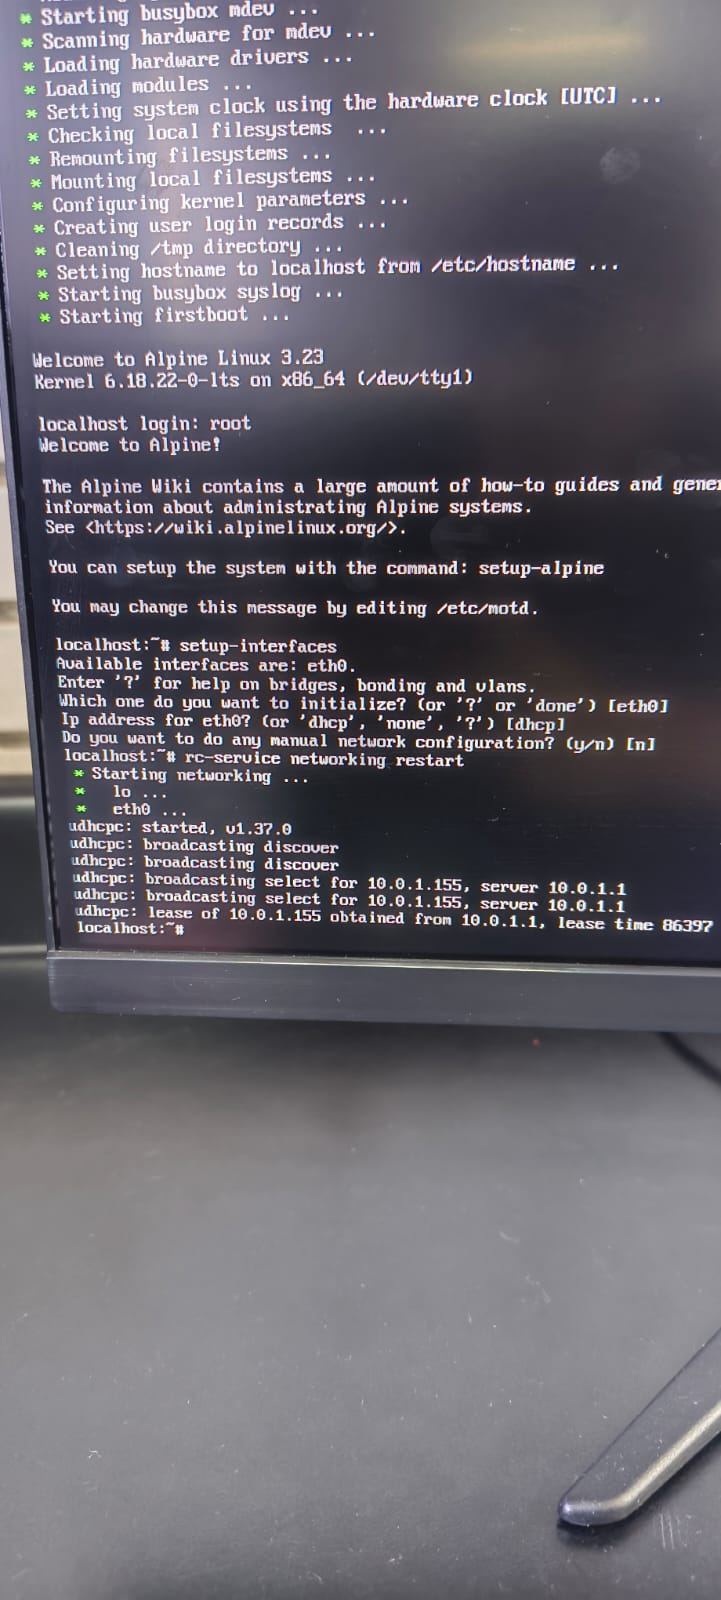
\includegraphics[width=.9\linewidth]{./2.jpg}
\end{center}

Una vez hecho esto, corremos:

\begin{verbatim}
rc-service networking restart
\end{verbatim}

Para cargar las configuraciones.

Una vez hecho esto, configuramos la lista de repositorios remotos de la cual nuestro sistema Live obtendrá los paquetes. Esto lo hacemos con:

\begin{verbatim}
setup-apkrepos
\end{verbatim}

Hecho esto, podemos comenzar a trabajar.
\subsection{Creación de las particiones necesarias}
\label{sec:orgf9b1fb8}

Alpine Linux, al igual que distribuciones dedicadas a correr en ambientes reducidos como Arch Linux no tiene un programa de instalación con interfaz gráfica. En su lugar, su imágen de instalación en realidad es una Live USB que carga el sistema en memoria y desde ahí nos permite tanto trabajar como instalarlo en un disco duro.

En esta live USB existen dos scripts dedicados a la instalación del sistema:

\begin{itemize}
\item setup-alpine
\item setup-disk
\end{itemize}

El primer script es un asistente de instalación interactivo (TUI) que nos irá haciendo preguntas para instalar Alpine. El problema de este script es que espera un disco completo para realizar su instalación, ya que realiza el particionado automáticamente.

Entonces, usaremos el segundo script. El cual espera un sistema raíz ya montado y preparado en \textbf{\emph{mnt}} para funcionar.

Vamos a preparar tres particiones: la partición raíz, la partición swap y la partición \textbf{/boot}, esta última preparada para arranque en UEFI, que es el arranque para el que están preparadas las computadoras de este laboratorio.

Repartiendo 64GB de almacenamiento entre estas particiones, asignamos los siguientes tamaños:

\begin{center}
\begin{tabular}{ll}
\hline
Particion & Tamaño asignado\\
\hline
Boot & 1GB\\
\hline
Root & 59GB\\
\hline
Swap & 4GB\\
\hline
\end{tabular}
\end{center}
\subsubsection{Preparación}
\label{sec:orgb728c1e}

Alpine Linux viene solamente con la versión de busybox de fdisk. Esta versión no nos resulta útil, ya que solo nos permite trabajar con tablas MBR. Instalaremos cfdisk con:

\begin{verbatim}
apk add cfdisk
\end{verbatim}
\subsubsection{Particiones}
\label{sec:orgcdf593b}

Secuencialmente vamos construyendo las particiones en el tamaño y formatos necesarios con la herramienta cfdisk. Esta herramienta resulta bastante intuitiva. Al final, nos queda la siguiente estructura:

\begin{center}
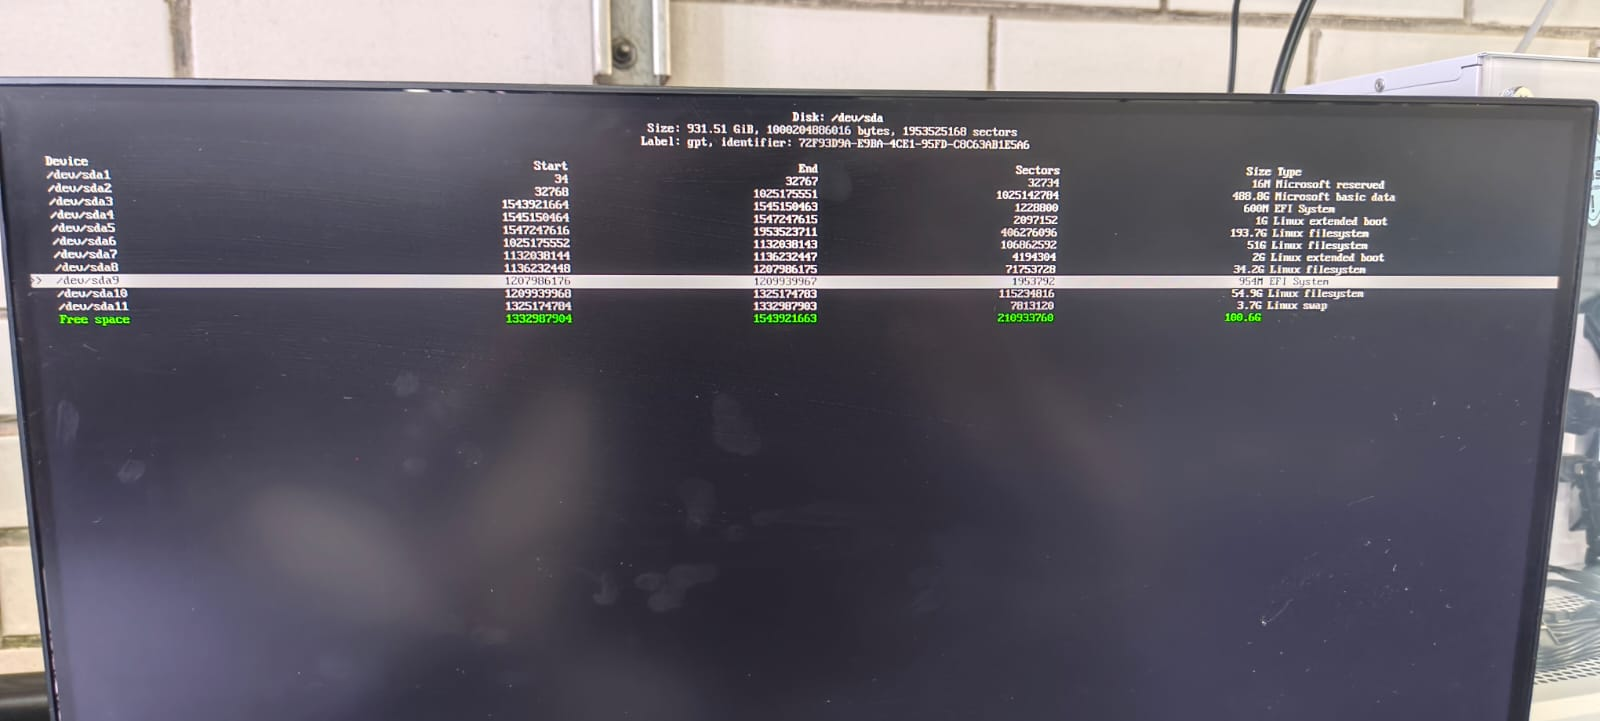
\includegraphics[width=.9\linewidth]{./3.jpg}
\end{center}
\subsubsection{Sistemas de archivos}
\label{sec:org39241f5}

Una vez creadas las particiones, creamos los sistemas de archivos según lo siguiente:

\begin{itemize}
\item Necesitamos que la partición boot sea de tipo FAT
\item La partición raíz debe ser de tipo ext4
\item La partición swap de tipo swap
\end{itemize}

Corriendo los siguientes comandos para hacer el sistema de archivos:

\begin{center}
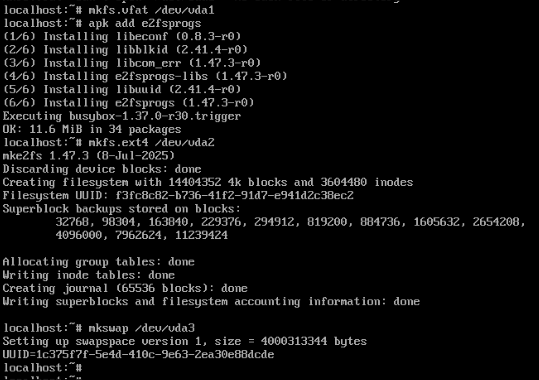
\includegraphics[width=.9\linewidth]{./4.png}
\end{center}

Error: el comando correcto para la partición de boot es:

\begin{verbatim}
mkfs.vfat -F32 <particion>
\end{verbatim}

Con esto, finalizamos la preparación de las particiones y los sistemas de archivos correspondientes. Por ende, la preparación para instalar el sistema Alpine Linux.
\section{Debian}
\label{sec:orga7b55d0}

\subsection{Despejar espacio para la instalación}
\label{sec:org78c2c0c}

Al disco NVME no hay que tocar nada. Debemos reducir alguna de las particiones ya existentes en el disco de estado sólido para realizar nuestra instalación.

En mi caso concreto, reduje /dev/sda8 para obtener 160GB de espacio disponibles. De los cuales 64GB los usé previamente para instalar Alpine Linux, el resto de este espacio despejado queda disponible para hacer las particiones en el instalador de Debian

\begin{center}
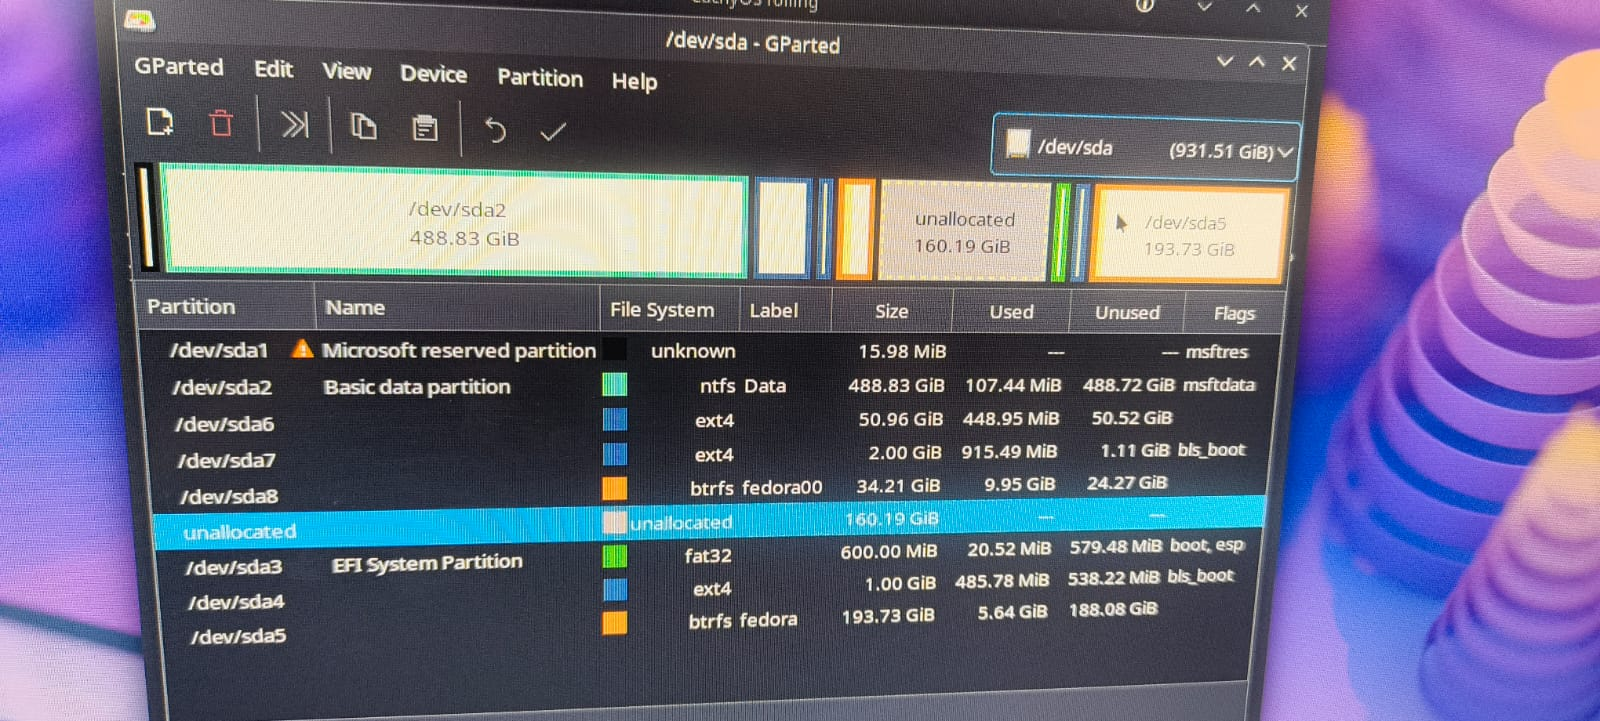
\includegraphics[width=.9\linewidth]{./1.jpg}
\end{center}
\subsection{Creación de las particiones necesarias}
\label{sec:org18adff2}

Debian tiene un asistente bastante funcional para crear las particiones deseadas en el sistema. Sobre este asistente, construyo las siguientes particiones de los siguientes tamaños

\begin{center}
\begin{tabular}{ll}
\hline
Particion & Tamaño asignado\\
\hline
Boot & 1GB\\
\hline
Root & 29GB\\
\hline
Swap & 2GB\\
\hline
\end{tabular}
\end{center}

Con esto, podemos proceder a la instalación.
\section{Redhat Enterprise Linux}
\label{sec:orgb584fad}

Vas mari
\section{Fedora}
\label{sec:org823ab2b}

Vas mari x2
\section{Bibliografía}
\label{sec:orga9011da}

\begin{itemize}
\item (S/f-a). Alpinelinux.org. Recuperado el 20 de mayo de 2026, de \url{https://wiki.alpinelinux.org/wiki/Repositories}

\item (S/f-b). Alpinelinux.org. Recuperado el 20 de mayo de 2026, de \url{https://wiki.alpinelinux.org/wiki/UEFI}

\item (S/f-c). Alpinelinux.org. Recuperado el 20 de mayo de 2026, de \url{https://wiki.alpinelinux.org/wiki/Alpine\_Package\_Keeper}

\item (S/f-d). Alpinelinux.org. Recuperado el 20 de mayo de 2026, de \url{https://wiki.alpinelinux.org/wiki/Setting\_up\_disks\_manually}

\item (S/f-e). Alpinelinux.org. Recuperado el 20 de mayo de 2026, de \url{https://wiki.alpinelinux.org/wiki/System\_Disk\_Mode}

\item (S/f-f). Alpinelinux.org. Recuperado el 20 de mayo de 2026, de \url{https://wiki.alpinelinux.org/wiki/Configure\_Networking}

\item (S/f-g). Alpinelinux.org. Recuperado el 20 de mayo de 2026, de \url{https://wiki.alpinelinux.org/wiki/Installation}

\item (S/f-h). Alpinelinux.org. Recuperado el 20 de mayo de 2026, de \url{https://wiki.alpinelinux.org/wiki/Filesystems}

\item (S/f-i). Alpinelinux.org. Recuperado el 20 de mayo de 2026, de \url{https://wiki.alpinelinux.org/wiki/Dualbooting}

\item (S/f-j). Alpinelinux.org. Recuperado el 20 de mayo de 2026, de \url{https://wiki.alpinelinux.org/wiki/Swap}
\end{itemize}
\end{document}
